%%%%%%%%%%%%%%%%%%%%%%%%%%%%%%%%%%%%%%%%%%%%%%%%%%%%%%%%%%%%%%%%%%%%%%%
%% Optionen zum Layout des Artikels                                  %%
%%%%%%%%%%%%%%%%%%%%%%%%%%%%%%%%%%%%%%%%%%%%%%%%%%%%%%%%%%%%%%%%%%%%%%%
\documentclass[%
  %a5paper,
]
{scrartcl}

%\pagestyle{empty}		% keine Kopf und le (k. Seitenzahl)
%\pagestyle{headings}	% lebender Kolumnentitel


%% Deutsche Anpassungen %%%%%%%%%%%%%%%%%%%%%%%%%%%%%%%%%%%%%
\usepackage[ngerman]{babel}
\usepackage[T1]{fontenc}
\usepackage[utf8]{inputenc}
\usepackage{amsmath}
\usepackage{amsfonts}
\usepackage{amssymb}
\usepackage{lmodern} %Type1-Schriftart
%Für das verlinkte Inhaltsverzeichnis
\usepackage[colorlinks,pdfpagelabels,pdfstartview = FitH,bookmarksopen = true,bookmarksnumbered = true,linkcolor = black,plainpages = false,hypertexnames = false,citecolor = black] {hyperref}
\usepackage{wrapfig}

%
\usepackage{graphicx} %%Zum Laden von Grafiken
\usepackage{subfig} %%Teilabbildungen in einer Abbildung
%\usepackage{tikz} %%Vektorgrafiken aus LaTeX heraus erstellen

\relpenalty=9999	%verhindert Trennung von $...$
\binoppenalty=9999


%% Bibliographiestil %%%%%%%%%%%%%%%%%%%%%%%%%%%%%%%%%%%%%%%%%%%%%%%%%%
%\usepackage{natbib}

\begin{document}



%%%%%%%%%%%%%%%%%%%%%%%%%%%%%%%%%%%%%%%%%%%%%%%%%%%%%%%%%%%%%%%%%%%%%%%
%% Ihr Artikel                                                       %%
%%%%%%%%%%%%%%%%%%%%%%%%%%%%%%%%%%%%%%%%%%%%%%%%%%%%%%%%%%%%%%%%%%%%%%%

%% eigene Titelseitengestaltung %%%%%%%%%%%%%%%%%%%%%%%%%%%%%%%%%%%%%%%
%\begin{titlepage}

%\end{titlepage}

%% Angaben zur Standardformatierung des Titels %%%%%%%%%%%%%%%%%%%%%%%%
%\titlehead{Titelkopf }
%\subject{Typisierung}
\title{Das Ising-Modell mit Monte-Carlo und Metropolis}
\author{Christian Darsow-Fromm
\and{Maximilian Menzel}}
%\publishers{Herausgeber}

%% Widmungsseite %%%%%%%%%%%%%%%%%%%%%%%%%%%%%%%%%%%%%%%%%%%%%%%%%%%%%%
%\dedication{Widmung}

\maketitle 						% Titelei wird erzeugt

%% Zusammenfassung nach Titel, vor Inhaltsverzeichnis %%%%%%%%%%%%%%%%%


%% Erzeugung von Verzeichnissen %%%%%%%%%%%%%%%%%%%%%%%%%%%%%%%%%%%%%%%
\tableofcontents			% Inhaltsverzeichnis
%\listoftables				% Tabellenverzeichnis
%\listoffigures				% Abbildungsverzeichnis

\setlength{\tabcolsep}{10pt}
\renewcommand{\arraystretch}{2}

%% Der Text %%%%%%%%%%%%%%%%%%%%%%%%%%%%%%%%%%%%%%%%%%%%%%%%%%%%%%%%%%%

\section{Das Ising-Modell}
Das Ising-Modell ist eine Vereinfachung des Heisenberg-Modells. Die Spins werden nicht als Vektor behandelt, sondern auf $s_i^z = \pm 1$ reduziert.
\begin{equation}
  \hat{\mathcal H} = -\frac 12\sum _{ij} J_{ij} s_i^z s_j^z - B_z \sum_{i=1}^N s_i^z
\end{equation}
%TODO schöne Einleitung
Deshalb ist das Ising-Modell vor allem dann eine gute Näherung des Heisenberg-Modells, wenn sich durch Anisotropien eine vorgezogene Richtung ergibt, oder wenn sich die Spins an einem Isotropen äußeren Magnetfeld ausrichten.
Um das Modell weiter zu vereinfachen, wird in der Regel für $J_{ij}$ eine nächste-Nachbar-Wechselwirkung angenommen. $J$ ist konstant für das gesamte System und es wird nur die Wechselwirkung mit den direkten Nachbarn berechnet.

Mit dem Modell kann der Phasenübergang eines Ferromagneten in zwei und mehr Dimensionen beschrieben werden.
\section{Die Monte-Carlo-Methode}
\label{sec:MonteCarloMethode}
Die Monte-Carlo-Methode ermöglicht das Simulieren von Systemen, die auf Wahrscheinlichkeiten beruhen.
Mit ihrer Hilfe ist es nicht nötig, komplexe stochastische Formeln zu entwickeln, sondern es reicht ein Zufallszahlengenerator aus.
Durch sehr häufige Wiederholung der Messung lassen sich gute statistische Näherungen simulieren.
Statistische Messungenauigkeiten dieser Simulationsmethode lassen sich auch bei realen Messungen beobachten. Daher ist Monte-Carlo relativ realitätsnah.

\paragraph{Monte-Carlo und Ising}
%TODO gegebenes Datenschema
Die Vereinigung von Monte-Carlo mit dem Ising-Modell funktioniert nach folgendem Schema:
\begin{enumerate}
 \item Wähle zufällig irgendeinen Spin $S_i$ aus und versuche ihn umzudrehen.

 \item Berechne die Energiedifferenz
		\begin{equation}
		  \Delta E = E(-S_i) - E(S_i) \label{eq:EnergieDiff}
		\end{equation}
		Wenn $\Delta E$ negativ ist, wird der Spinflip akzeptiert.
		Ansonsten wird die Entscheidung Metropolis überlassen.\\
		\textbf{Metropolis:} Wähle eine Zufallszahl $r$ zwischen $0$ und $1$.
		Wenn
		\begin{equation}
		  r<e^{-\beta \Delta E} \label{eq:FlipChance}
		\end{equation}
		wird der Flip akzeptiert. $\beta=\frac{1}{k_B T}$ also der Kehrwert der Temperatur $T$, da bei uns die Boltzmann-Konstante $k_B$ gleich eins ist.

 \item Speichere die neue Wahrscheinlichkeit der Spinausrichtung
		\begin{equation}
		  \langle S_i \rangle_{\text{neu}} = \frac{\langle S_i \rangle \cdot N_i + S_i}{N_i + 1},  \label{eq:RekursiverMittelwert}
		\end{equation}
		wobei $N_i$ die Anzahl der bisherigen Messungen des Spins $S_i$ ist.

 \item Die Magnetisierung $M$ ist die Summe der Erwartungswerte der einzelnen Spins $S_i$, normalisiert mit der Anzahl der Spins $N$:
		\begin{equation}
		  M = \frac 1N \sum_i \langle S_i \rangle \label{eq:MagErwartungswert}
		\end{equation}
\end{enumerate}
Die Punkte eins bis drei werden immer wiederholt und zum Schluss die Magnetisierung gemessen.

\section{Die Implementierung}
blabla

\section{Simulations-Ergebnisse}

\subsection{Der kritische Punkt}
\begin{wrapfigure}[19]{r}{8.5cm}
  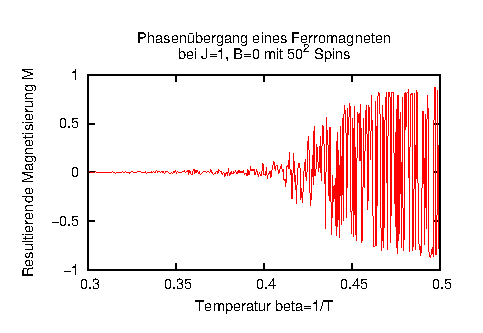
\includegraphics[width=0.6\textwidth]{bilder/critical/critical.eps}
  \caption{Phasenübergang eines Ferromagneten. Die Simulation ging mit 400 Schritten von $\beta=0.3$ bis $\beta=0.5$ \label{phase}}
\end{wrapfigure}
Ferromagneten zeigen bei einer bestimmten Temperatur einen Phasenübergang. Wenn die Temperatur einen kritischen Wert unterschreitet, kann eine spontane Magnetisierung einsetzen.
Das Ising-Modell hat diesen Phasenübergang bei zwei Dimensionen und mehr. In einer Dimension gibt es zu wenige nächste Nachbarn.

Abbildung \ref{phase} zeigt, wie ab einer Temperatur von $\beta=1/T\approx0.4$ die spontane Magnetisierung einsetzt.
Die Simulation wurde mit $50^2$ Spins, ohne Magnetfeld und für jedes der $400$ verschiedenen $\beta$ mit $6\cdot10^6$ Monte-Carlo-Schritten durchgeführt.
Man kann gut sehen, dass die Magnetisierung mit zunehmendem $\beta$ immer stärker ausschlägt und bei fast jeder Messung annähernd die Sättigung erreicht wird.
Dabei ist es vollkommen zufällig, in welche Richtung der Magnet ausgerichtet ist.


\subsection{Hysterese beim Ferromagneten}
\begin{wrapfigure}[16]{r}{8.5cm}
  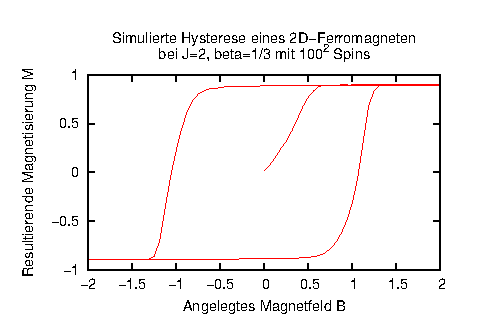
\includegraphics[width=0.6\textwidth]{bilder/hysterese/hysterese.eps}
  \caption{Hysterese eines Ferromagneten. Die Simulation ging mit 400 Schritten: $B=0\to 5 \to -5 \to 5$\label{hysterese}}
\end{wrapfigure}
Ein Ferromagnet widersteht einem wechselnden äußeren Magnetfeld, bevor er selbst seine Ausrichtung ändert.
Diese Hysterese lässt sich auch mit dem Ising-Modell gut beschreiben.

Für die Simulation haben wir wieder $100^2$ Spins mit einer ferromagnetischen Wechselwirkung von $J=2$.
Die Temperatur ist mit $\beta=\frac 13$ klein genug für die ferromagnetische Phase.
Das externe Magnetfeld läuft von $B=0$ bis zur Sättigung $B=5$, anschließend bis $B=-5$ und noch einmal ins Positive.
Dabei wird $B$ in 400 Einzelschritten linear geändert und mit jeweils $10^5$ Monte-Carlo-Schritten stabilisiert.
Das Ergebnis (Abbildung \ref{hysterese}) zeigt einen relativ glatten Verlauf und die Rechenzeit hielt sich mit 21 Sekunden in Grenzen, so dass wir bislang keine weitere Geschwindigkeitsoptimierung vorgenommen haben.

\begin{figure}[h]
    \subfloat{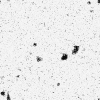
\includegraphics[width=0.15\textwidth]{bilder/hysterese/b_169.png}}
  \hfill
    \subfloat{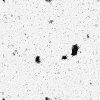
\includegraphics[width=0.15\textwidth]{bilder/hysterese/b_170.png}}
  \hfill
    \subfloat{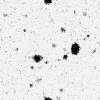
\includegraphics[width=0.15\textwidth]{bilder/hysterese/b_171.png}}
  \hfill
    \subfloat{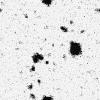
\includegraphics[width=0.15\textwidth]{bilder/hysterese/b_172.png}}
  \hfill
    \subfloat{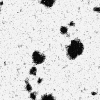
\includegraphics[width=0.15\textwidth]{bilder/hysterese/b_173.png}}
  \hfill
    \subfloat{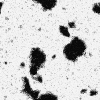
\includegraphics[width=0.15\textwidth]{bilder/hysterese/b_174.png}}
  \\
    \subfloat{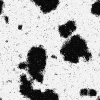
\includegraphics[width=0.15\textwidth]{bilder/hysterese/b_175.png}}
  \hfill
    \subfloat{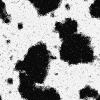
\includegraphics[width=0.15\textwidth]{bilder/hysterese/b_176.png}}
  \hfill
    \subfloat{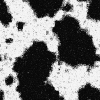
\includegraphics[width=0.15\textwidth]{bilder/hysterese/b_177.png}}
  \hfill
    \subfloat{
\includegraphics[width=0.15\textwidth]{bilder/hysterese/b_178.png}}
  \hfill
    \subfloat{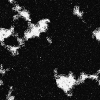
\includegraphics[width=0.15\textwidth]{bilder/hysterese/b_179.png}}
  \hfill
    \subfloat{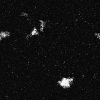
\includegraphics[width=0.15\textwidth]{bilder/hysterese/b_180.png}}
\caption{Ausrichtungswahrscheinlichkeiten der Spins beim Richtungswechsel der Hysteresekurve.\label{hysterese-wechsel}}
\end{figure}

Der Übergang von positiver zu negativer Magnetisierung der Hysteresekurve ist nochmal in Bildern in Abbildung \ref{hysterese-wechsel} zu sehen.
Hier sind die Mittelwerte der einzelnen Spins (ein Spin pro Pixel) wie in Abbildung \ref{domainwall} (a) zu sehen.
Man kann gut die zufälligen Strukturen erkennen, die sich beim Übergang ergeben.
Bestehende Flächen von Spins, die schon negativ (schwarz) ausgerichtet sind, werden immer größer und breiten sich immer weiter aus.


\subsection{Domänenwände beim Antiferromagneten}
Bei geringen Temperaturen gibt es in einem Antiferromagneten nur noch sehr wenige Störstellen.
Da sich das \textit{Schachbrettmuster} beim Abkühlen von mehreren Stellen gleichzeitig ausbreitet, bleiben am Ende einige Stellen übrig, an denen es unterbrochen ist. Diese Domänenwände haben eine Breite von genau zwei Spins, die nebeneinander die gleiche Ausrichtung haben.
Es wäre energetisch viel aufwändiger, einen ganzen Bereich mit \textit{falscher} Ausrichtung umzudrehen, als diese dünnen Wände stehen zu lassen.
\begin{figure}[h]
  \subfloat[Mittelwerte der Spins]{
\includegraphics[width=200pt]{bilder/domainwall/beta_1.png}}
  \hfill
  \subfloat[Letzte Spin-Konfiguration der Messung]{
\includegraphics[width=200pt]{bilder/domainwall/spins_1.png}}
  \caption{Domänenwände eines Antiferromagneten bei $\beta\approx 345, J=-1, B=0$\label{domainwall}}
\end{figure}

Obwohl die Simulation bei uns mit konstanter Temperatur abläuft, wird praktisch eine Abkühlung simuliert.
Die Startkonfiguration ist eine Zufallsverteilung, die einer hohen Temperatur entspricht.

Abbildung \ref{domainwall} zeigt eine Beispielsimulation, bei der Domänenwände sichtbar werden.
Simuliert wurde in zwei Dimensionen mit $100^2$ Spins und ohne externes Magnetfeld.
Die Simulation ist nur eingeschränkt auf die Realität übertragbar, da die Grundannahme des Ising-Modells, dass Spins nur in einer Achse ausgerichtet sein können, ohne externes Magnetfeld natürlich nicht erfüllt ist.

Bei den Abbildungen weichen die Mittelwerte doch an einigen Stellen deutlich von der Momentaufnahme ab.
Um hier wirklich ein statisches Bild zu geben, scheint die Temperatur noch nicht niedrig genug zu sein.


%\bibliography{literatur}
%\bibliographystyle{alpha}
\end{document}
